\documentclass[11pt]{article}
\usepackage{color}
\usepackage{graphicx}
\usepackage{amsmath,amsthm,amssymb,multirow,paralist}
\usepackage[margin=0.8in]{geometry}
\usepackage{hyperref}

\begin{document}

\begin{center}
{\Large \textbf{COM S 573: Machine Learning}\\Homework \#3}\\

\linethickness{1mm}\line(1,0){498}

\begin{enumerate}
\item Please put required code files and report into a
compressed file ``HW\#\_FirstName\_LastName.zip''
\item Unlimited number of submissions are
allowed on Canvas and the latest one will be graded.
\item {\color{red} No later submission is accepted.}
\item Please read and follow submission instructions. No exception
will be made to accommodate incorrectly submitted files/reports.
\item All students are required to typeset their reports using
latex. Overleaf
(\url{https://www.overleaf.com/learn/latex/Tutorials}) can be a
good start.
\end{enumerate}

\linethickness{1mm}\line(1,0){498}

\end{center}

%%%%%%%%%%%%%%%%%%%%%%%%%%%%%%%%%%%%%%%%%%%%%%%%%%%%%%%%%%%%%%%%%%%%%%%%%%%%%%%

%%%%%%%%%%%%%%%%%%%%%%%%%%%%%%%%%%%%%%%%%%%%%%%%%%%%%%%%%%%%%%%%%%%%%%%%%%%%%%%


\begin{enumerate}

\item (15 points) You are provided with a training set of
examples (see Figure~\ref{fig:tree}). Which feature will you pick
first to split the data as per the ID3 decision tree learning
algorithm? Show all your work: compute the information gain for
all the four attributes and pick the best one.

\begin{figure*}[ht]\label{fig:tree}
\begin{center}
    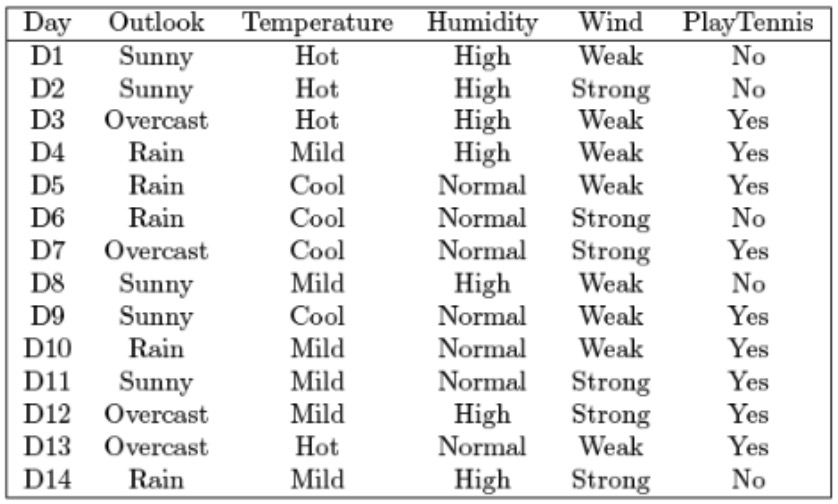
\includegraphics[width=0.6\textwidth]{FIG/tree.jpg}
    \caption{Table with training examples. Each row corresponds
    to a single training example. There are four features,
    namely, outlook, temperature, humidity, and wind.
    ``PlayTennis'' is the class label.}
\end{center}
\end{figure*}

\item (15 points) We know that we can convert any decision tree
into a set of if-then rules, where there is one rule per leaf
node. Suppose you are given a set of rules $R = \{r_1, r_2,
\dots, r_k\}$, where $r_i$ corresponds to the $i^{th}$ rule.
{\color{red} These rules are valid and complete, which means
there is no conflicting rules. You can always obtain a prediction
based on these rules.} Is it possible to convert the rule set $R$
into an equivalent decision tree? Explain your construction or
give a counterexample.


\item (20 points) Suppose $\boldsymbol x = [x_1, x_2, \dots,
x_d]$ and $\boldsymbol z = [z_1, z_2, \dots, z_d]$ be two points in
a high-dimensional space (i.e., $d$ is very large).

\begin{enumerate}
    \item (10 points) Try to prove the following, where the
    right-hand side quantity represent the standard Euclidean
    distance.
    \begin{align*}
        \left(\frac{1}{\sqrt{d}}\sum_{i=1}^d x_i - \frac{1}{\sqrt{d}} \sum_{i=1}^d z_i \right)^2 \le
        \sum_{i=1}^d \left(x_i - z_i\right)^2
    \end{align*}

    \textbf{Hint: } Use Jensen’s inequality – If $X$ is a random
    variable and $f$ is a convex function, then $f(E[X]) \le
    E[f(X)]$.

    
    \item (10 points) We know that the computation of nearest
    neighbors is very expensive in the high-dimensional space.
    Discuss how we can make use of the above property to make the
    nearest neighbors computation efficient?


\end{enumerate}

\item (50 points) \textbf{Fortune Cookie Classifier}: You will
build a binary fortune cookie classifier. This classifier will be
used to classify fortune cookie messages into two classes:
messages that predict what will happen in the future (class 1)
and messages that just contain a wise saying (class 0). For
example, ``Never go in against a Sicilian when death is on the
line'' would be a message in class 0. ``You will get an A in
Machine learning class'' would be a message in class 1.

\textbf{Files Provided:} There are three sets of files. All words
in these files are lower case and punctuation has been removed.

1) The training data: traindata.txt. This is the training data
consisting of fortune cookie messages. trainlabels.txt: This file
contains the class labels for the training data. 

2) The testing data: testdata.txt. This is the testing data
consisting of fortune cookie messages. testlabels.txt: This file
contains the class labels for the testing data. 

3) A list of stopwords: stoplist.txt 

There are two steps: the pre-processing step and the
classification step. In the pre-processing step, we convert
fortune cookie messages into features to be used by your
classifier. We use a bag of words representation. The following
steps outline the process involved: 

Form the vocabulary. The vocabulary consists of the set of all
the words that are in the training data with stop words removed
(stop words are common, uninformative words such as ``a'' and
``the'' that are listed in the file stoplist.txt). The vocabulary
will now be the features of your training data. Keep the
vocabulary in alphabetical order to help you with debugging. 

Then, we convert the training data into a set of features. Let M
be the size of your vocabulary. For each fortune cookie message,
we convert it into a feature vector of size M. Each slot in
that feature vector takes the value of 0 or 1. For these M slots,
if the ith slot is 1, it means that the ith word in the
vocabulary is present in the fortune cookie message; otherwise,
if it is 0, then the ith word is not present in the message. Most
of these feature vector slots will be 0. Since you are keeping
the vocabulary in alphabetical order, the first feature will be
the first word alphabetically in the vocabulary.

\begin{enumerate}
\item (20 points) Implement the ID3 decision tree learning
algorithm that we discussed in the class. The key step in the
decision tree learning is choosing the next feature to split on.
Implement the information gain heuristic for selecting the next
feature. Please see lecture notes or
\url{https://en.wikipedia.org/wiki/ID3_algorithm} for more
details.

\item (20 points) Implement the decision tree pruning algorithm
discussed in the class (via validation data).

\item (10 points) Compute the accuracy of decision tree and
pruned decision tree on validation examples and testing examples.
List your observations by comparing the performance of decision
tree with and without pruning.

\end{enumerate}


\end{enumerate}

\end{document}
